\section{问题三分析与求解}
\subsection{问题三分析}
\subsubsection{随机回退机制分析}

问题三是建立在问题一和问题二的基础上,题中提到对于MCS与NSS的对应取值可以参考在数据中实际测到的数据数值对,加上其他的特征值对AP的吞吐量进行模型的训练与预测。同时通过第四章模型准备中的流程分析,可以得知在数据发送过程中会发生一定的AP冲突,这会导致双方AP的回退时间增加,同时本是经过一定随即回退时间后要完成数据的传输,现在反而浪费了时间却没有增加AP的吞吐量,所以退回时间在一定程度上直接影响着AP的吞吐量,以及系统的吞吐量。

在过程中可以知道每一次回退时间的期望值为$\frac{(CW-1)\times slotTime}{2}$,则其如果发生数据传输冲突,则会对CW进行翻倍,这时候他的时间窗口为$\left[ 0,CW\times 2-1\right] $,那么这时候为第二次回退期望时间为$\frac{(CW\times 2-1)\times slotTime}{2}$,故第n次回退时间的期望是$\frac{(CW\times 2^{n-1}-1)\times slotTime}{2}$。但是当$CW$翻倍到$CW_{max}$的时候$CW$将不会变动,直到成功接收到$ACK$才会将$CW$进行重置,则需要计算其最小值$\frac{1}{2}min(CW\times 2^{n-1}-1,CW_{max}-1)\times slotTime$。

但是上述是对第n次回退时的回退时间期望的求解,而如果要从系统的角度看,需要去计算第n次回退时累计回退期望时长,即

\begin{equation}\label{eq1}
	backoffTime=\frac{1}{2}\sum_{i=1}^{n} min(CW\times 2^{i-1}-1,CW_{max}-1)\times slotTime
\end{equation}


\begin{figure}[htbp]
	\centering
	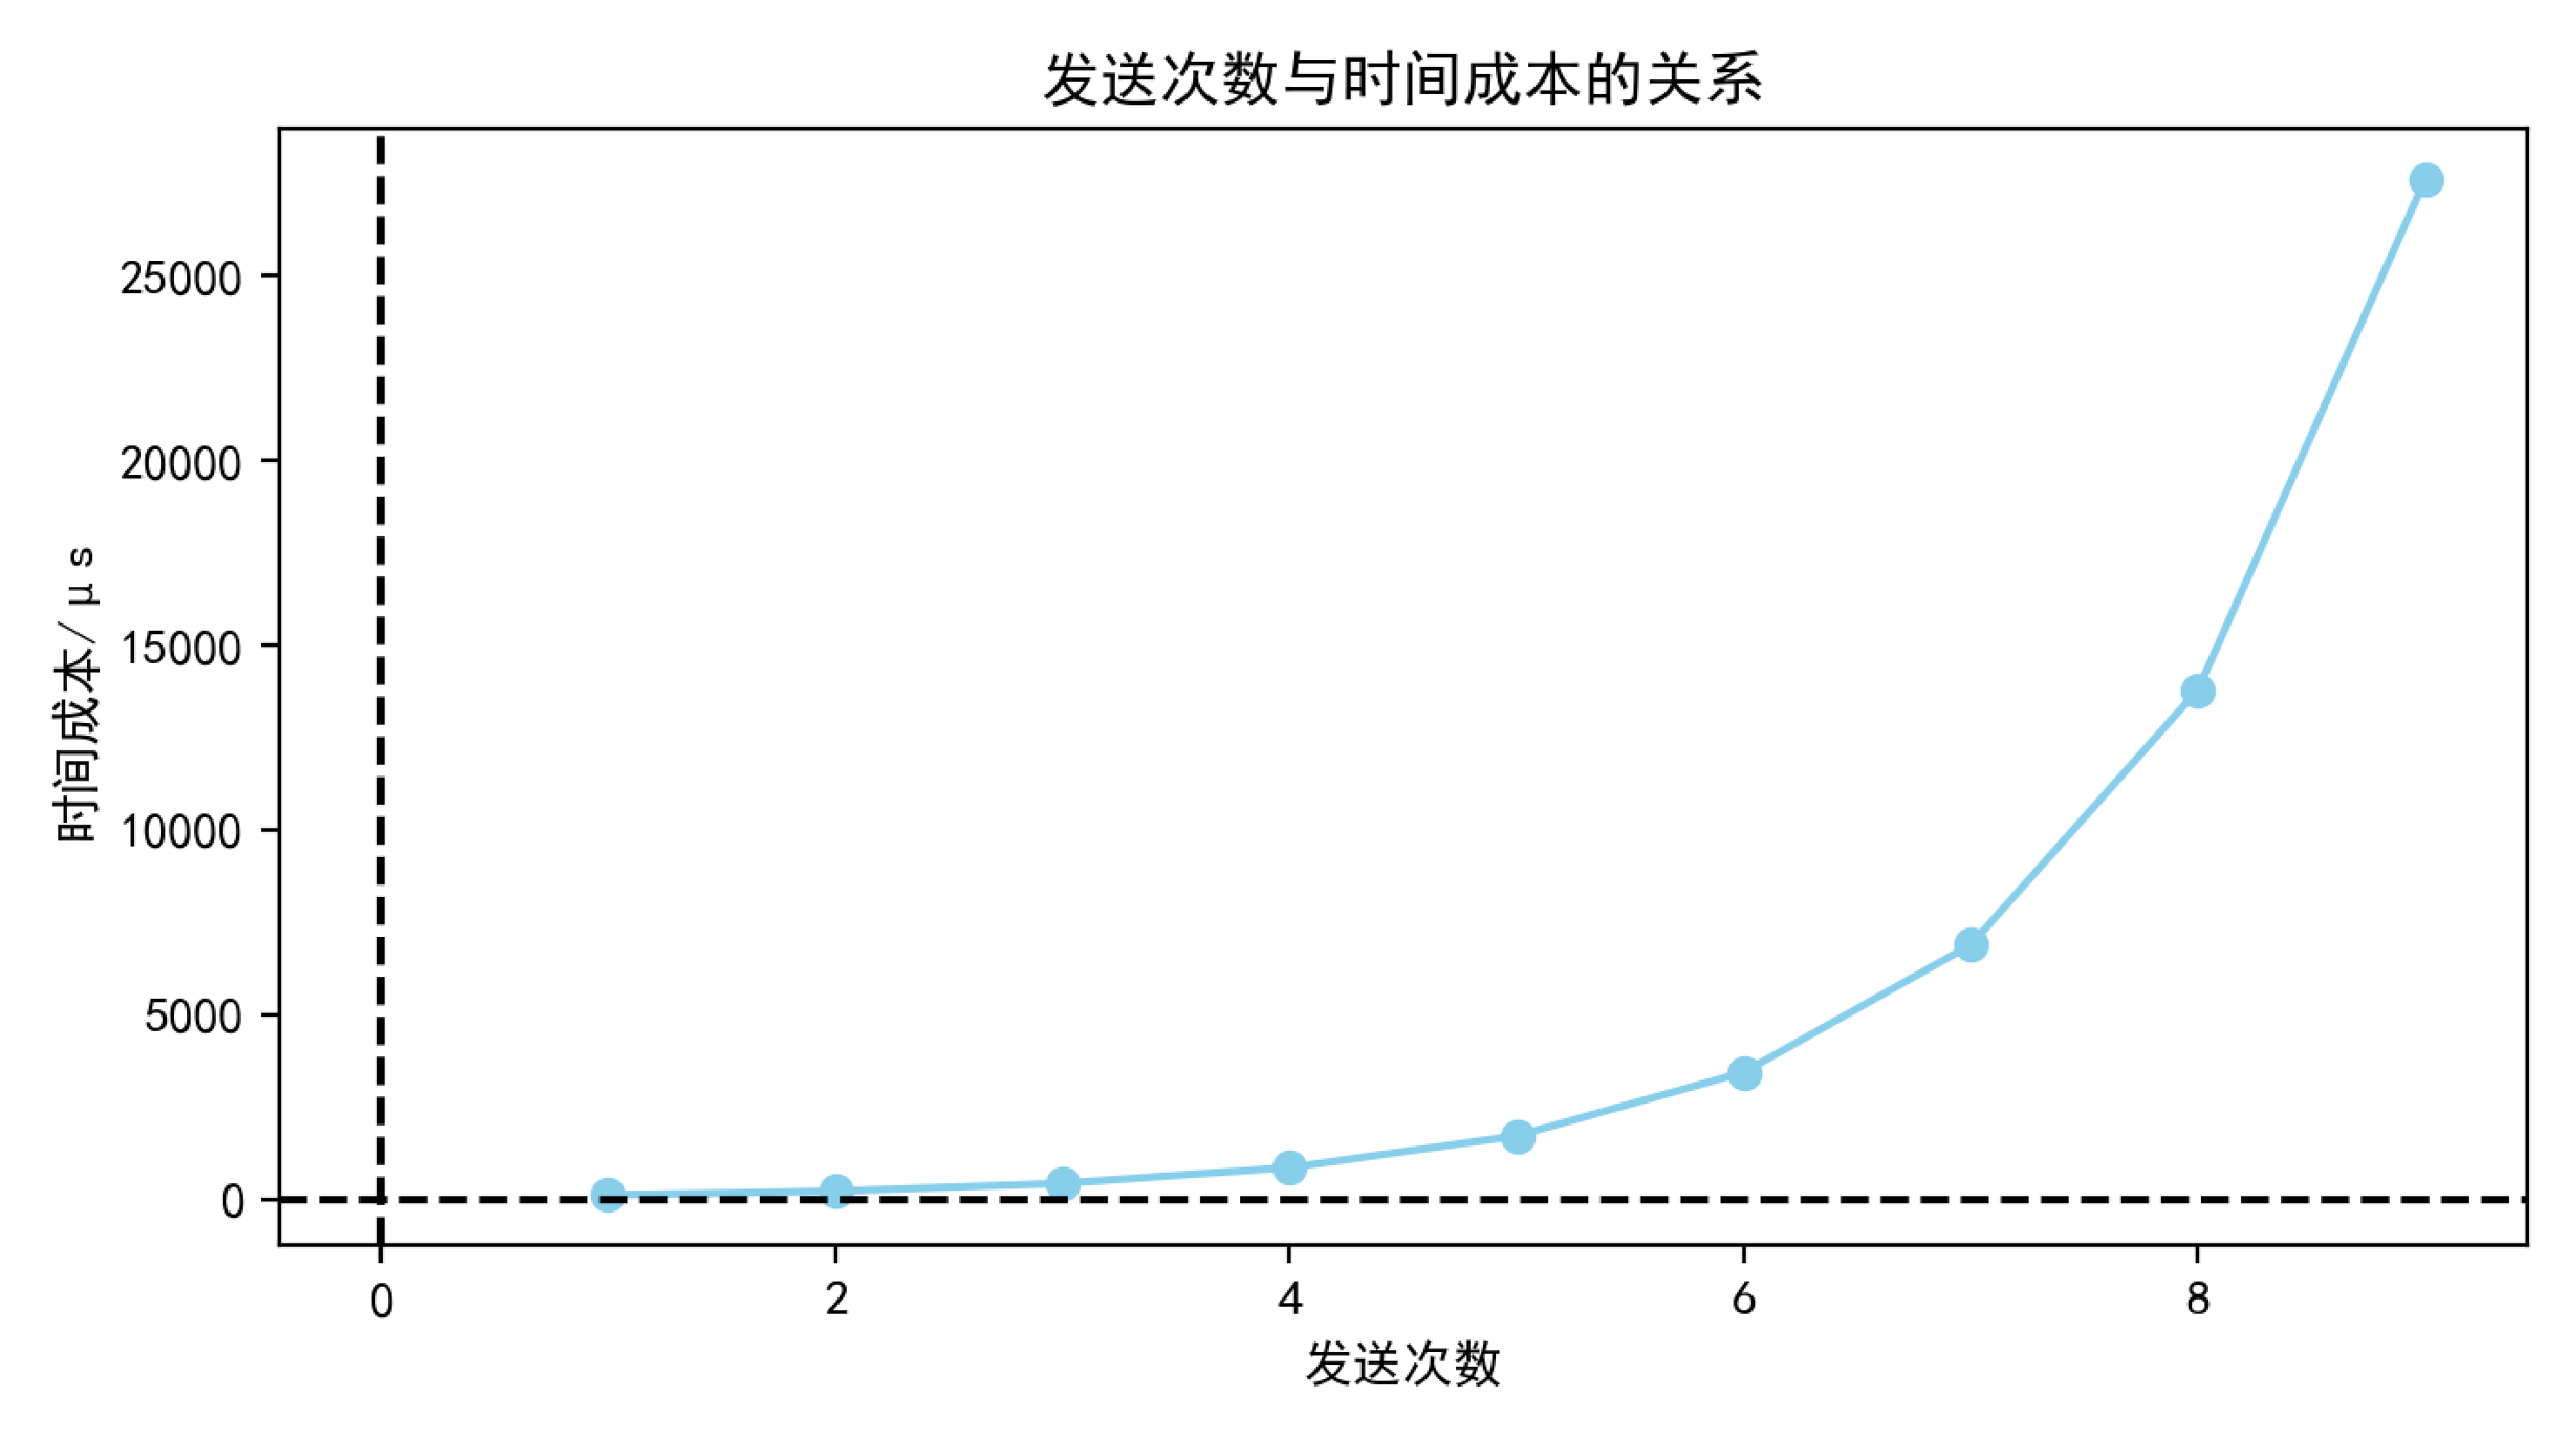
\includegraphics[width=0.75\linewidth]{2.eps}
	\caption{发送次数与时间成本折现图($ap\_num=2,CW_{min}=6,CW_{max}=2100$)}
	\label{figure2}
\end{figure}

同时第一次传输时随即回退时间窗格数量为$\frac{CW-1}{2}$,那么另一个AP在本AP随机回退的窗格数量中每一个停止的概率是相同的,所以另一个AP与本AP发生冲突的概率是$\frac{2}{CW-1}$,则等环境中一共有$ap\_Num$个AP时,他的冲突概率是$\frac{2(ap\_Num-1)}{CW-1}$,则其第n次不发生冲突的概率为

\begin{equation}
	P_{n}=1-\frac{2(ap\_Num-1)}{CW\times 2^{n-1}-1}
\end{equation}

\begin{figure}[H]
	\centering
	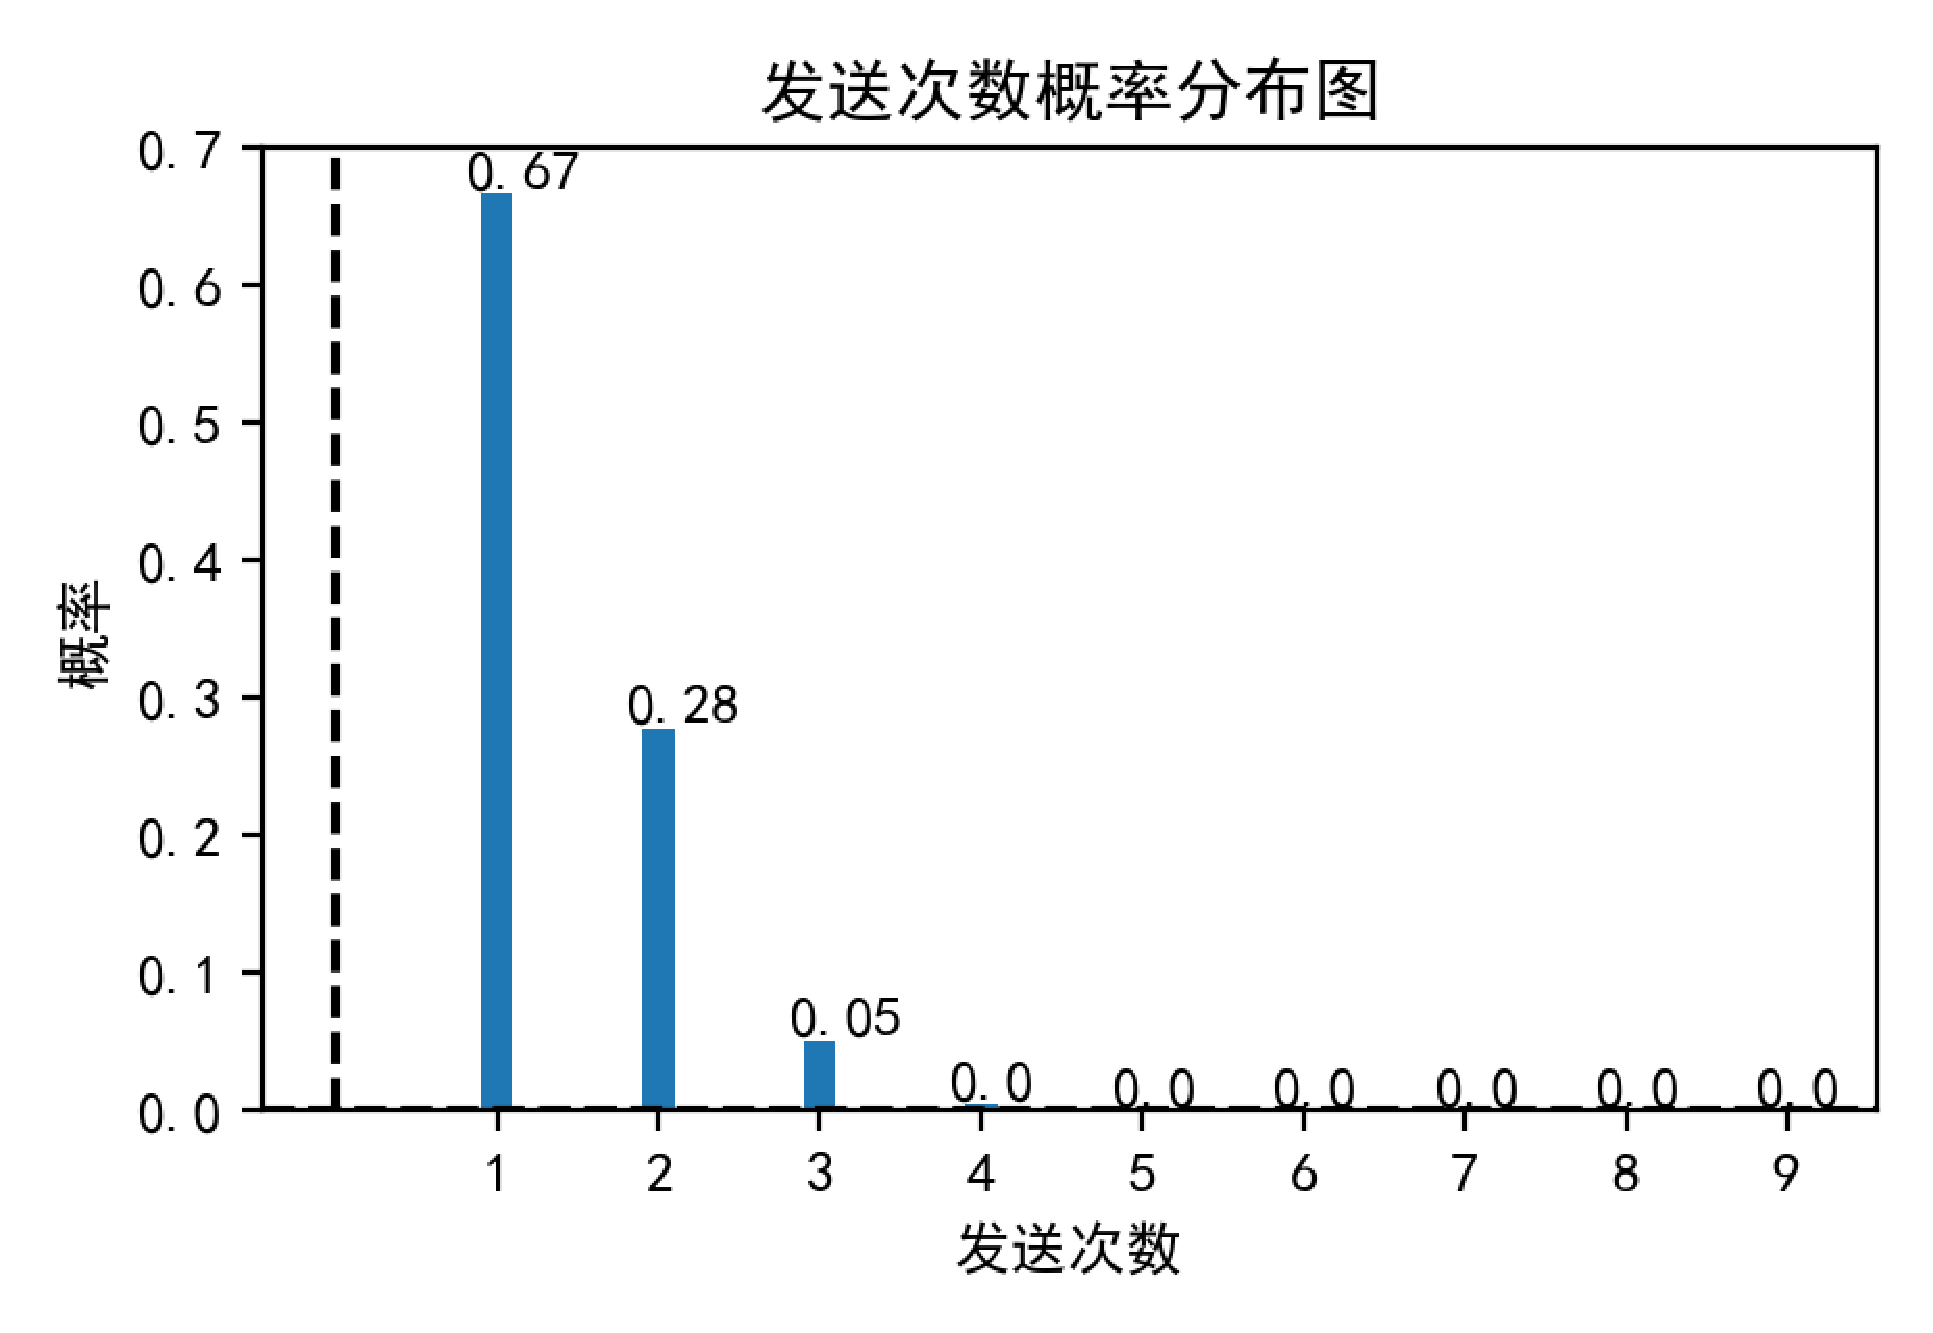
\includegraphics[width=0.75\linewidth]{1.eps}
	\caption{发送次数概率分布图($ap\_num=2,CW_{min}=6,CW_{max}=2100$)}
	\label{figure1}
\end{figure}


故当发生到第n次才能成功发送的概率服从以下分布:

\begin{equation}
	Pr_{(x=n)}=\prod_{i=1}^{n-1}{\left( 1-P_i \right) \times}P_n
\end{equation}

则可以利用$backoffTime$和$P_n$计算得到第n次期望的退回时间即新特征指标$BackMean$:

\begin{equation}
	BackMean=\sum_{i=1}^n{Pr_{(x=n)}\times backoffTime_i}
\end{equation}

\begin{figure}[H]
	\centering
	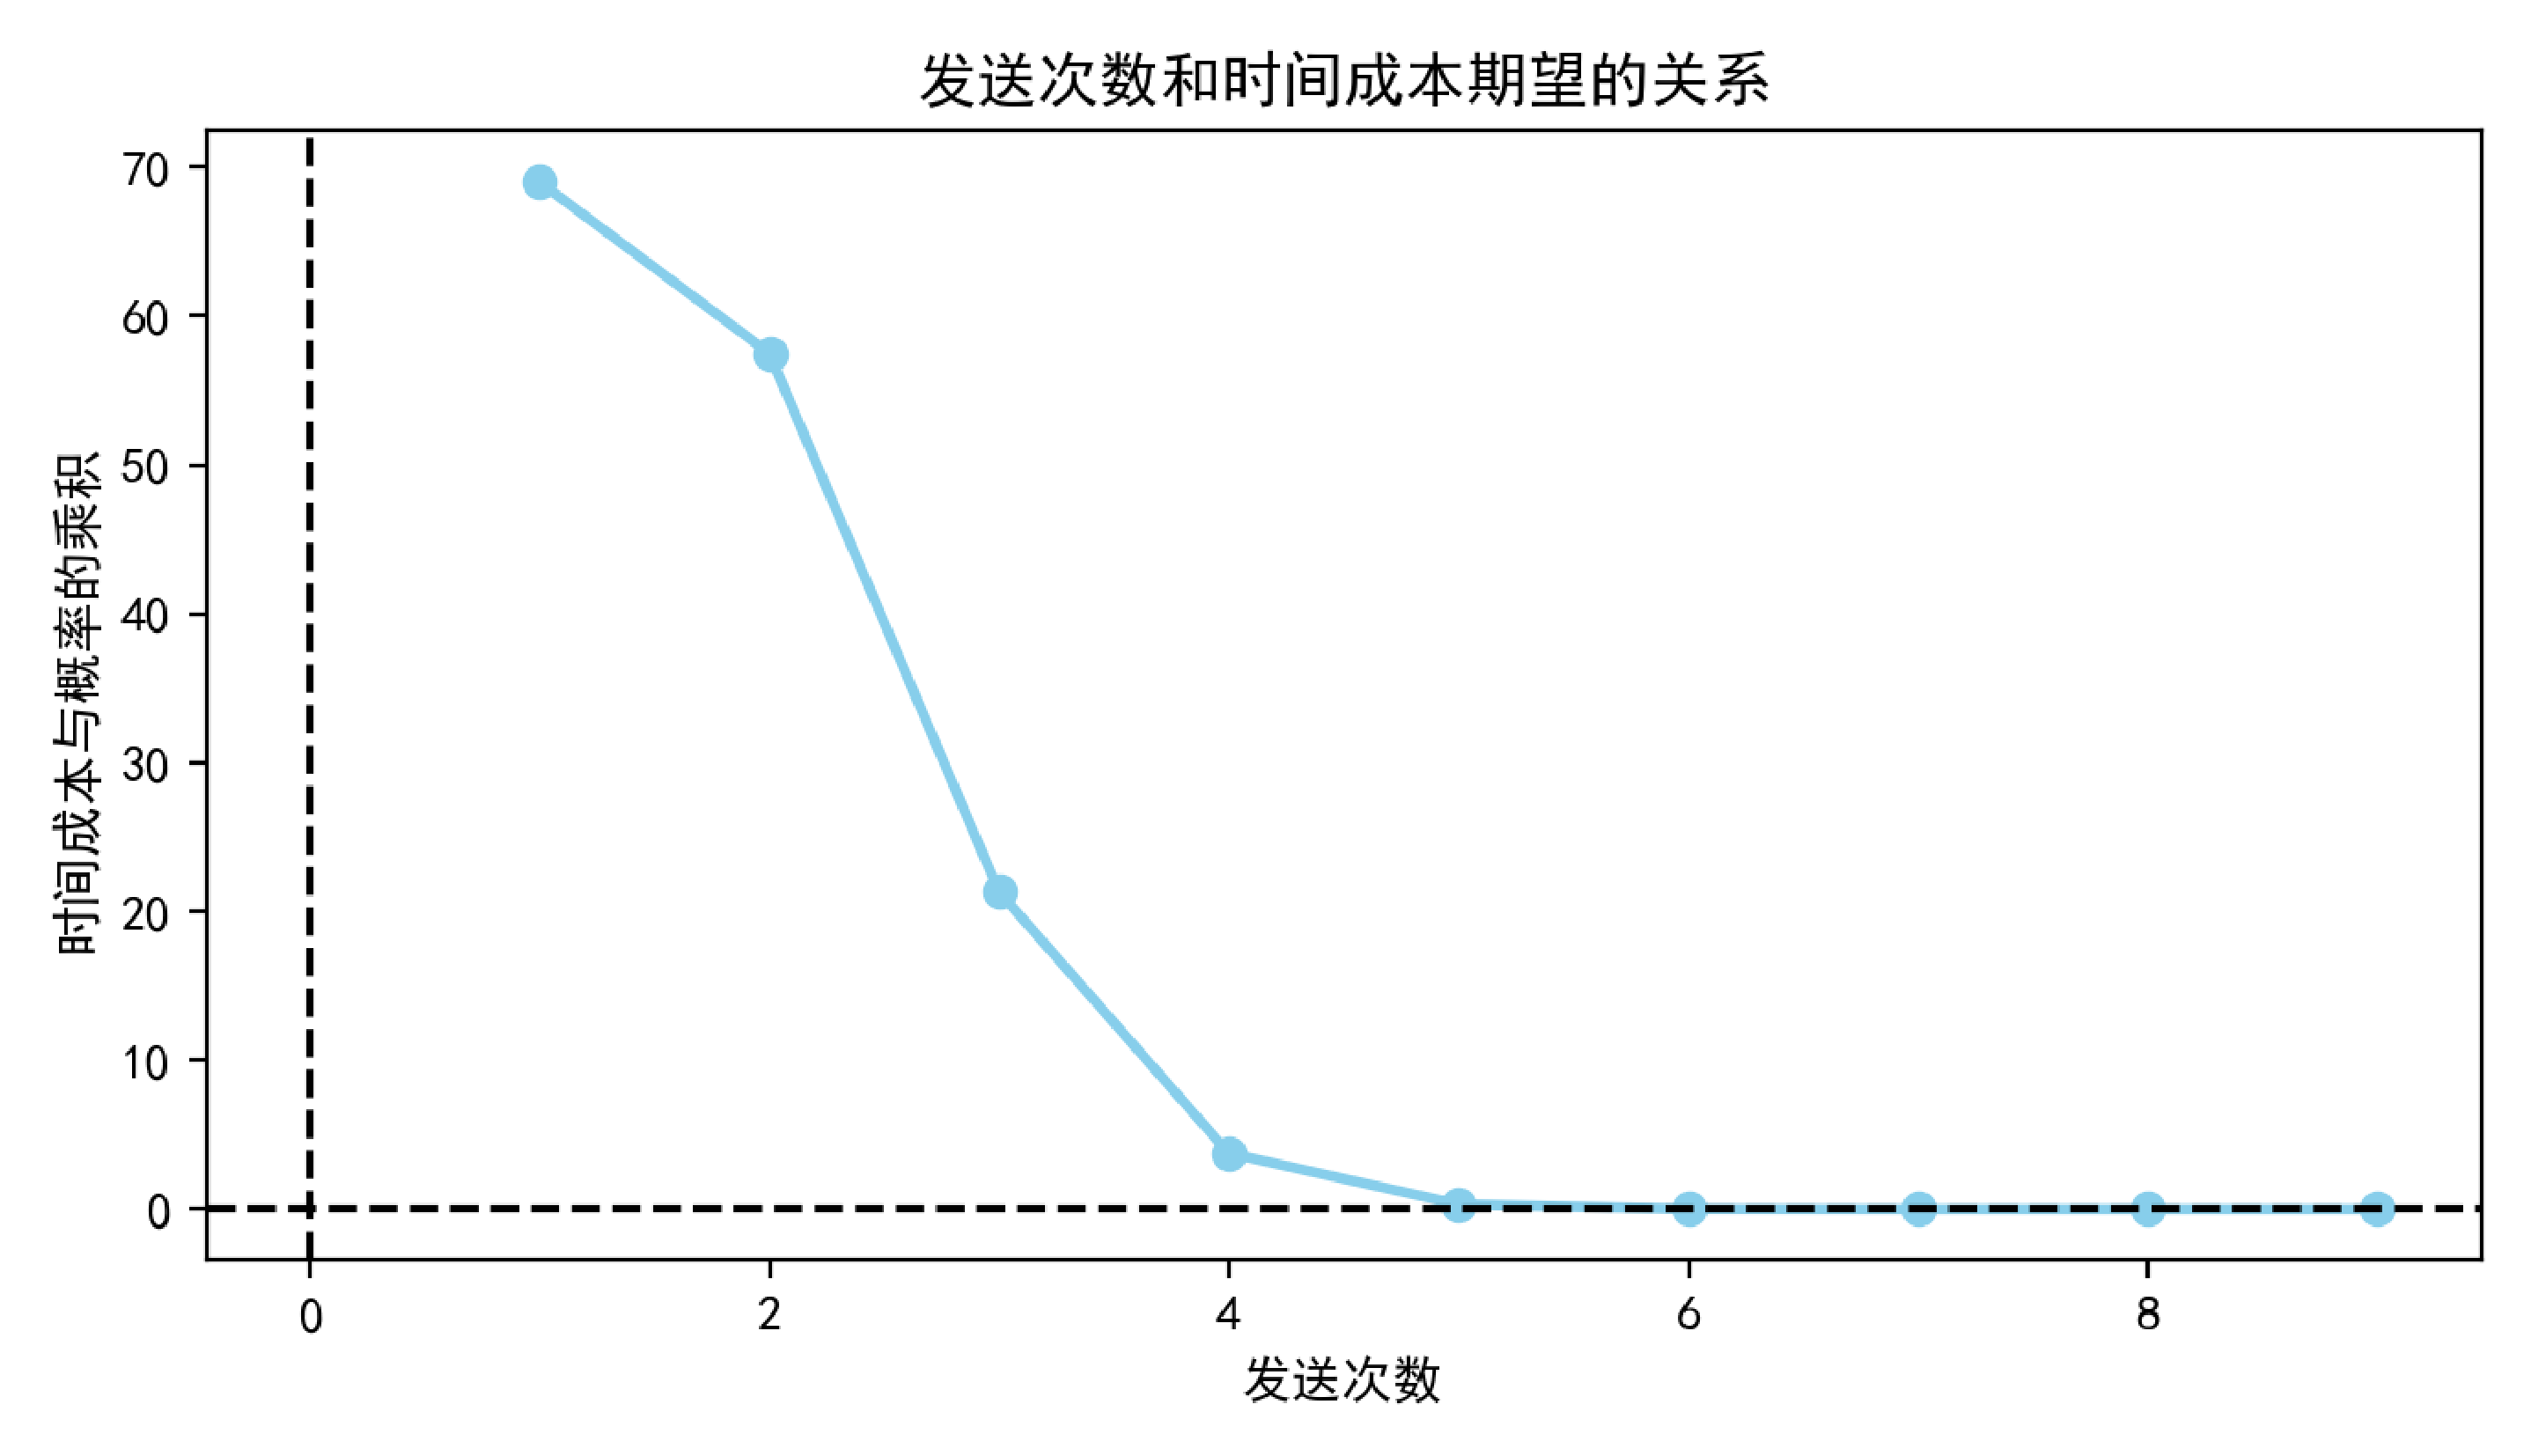
\includegraphics[width=0.75\linewidth]{figures/3}
	\caption{发送次数时间期望图($ap\_num=2,CW_{min}=6,CW_{max}=2100$)}
	\label{figure3}
\end{figure}

其再这种情形下,$ap\_num$为2,$CW_{min}$值为6,$CW_{max}$为2100个$slotTime$下,每次发送一个数据帧,所需等待时间151.9μs。

与随机回退机制息息相关的参数是per,丢包率这一项,丢包情况即不会收到确认帧情况,此时会让CW增加,以减少下一次发送数据冲突丢包。

\subsubsection{数据帧聚合策略分析}

在数据聚合策略中,存在两种聚合方式:ASMDU(A-MSDU Aggregation)和APMDU(A-MPDU Aggregation)。ASMDU在链路层进行聚合,而APMDU则在物理层实施。据相关资料指出,ASMDU聚合的上限通常由最大传输单元(MTU)和最大帧大小决定,其典型值为1500字节。根据802.11n标准,一个AMPDU的最大长度可达到65535字节。在数据集中,pkt\_len值为1500字节,即聚合前每一帧的数据长度,已达到ASMDU聚合的上限,因此无法采用ASMDU策略,只能选择APMDU策略。

多个PMDU(MAC Protocol Data Unit)通过聚合共享一个PHY(Physical Layer)头,以减少每次发送所必需的开销。换言之,每聚合一个数据帧,将减少一个PHY头的开销,PHY头在20MHz带宽中,大约需要传输20μs,而PHYRate最小为8.6Mbps,即最小的PHY头大约需要20*8.6=172bits=21.5bytes。然而,聚合需要进行0至3字节的填充对齐,其预期开销为1.5字节。此外,还需添加4字节的分隔符。因此,物理层每聚合一个PMDU,总体上最少可以减少16bytes花销。

故聚合次数越多,可以认为信道利用率越高,但是相应的per丢包率等也会增加,两者都会对吞吐量有很大的影响故并非聚合越多吞吐量越大。

在数据上体现聚合影响的参数就是ppdu\_dur,num\_ppdu,per这三个参数。

\subsection{问题三求解}
\subsubsection{特征构建}

根据题目与资料搜集可知,聚合过程会将多个数据包合并成一个,从而减少每个包的头部开销,提高有效负载的比例。合并数据包可以减少传输中的延迟和等待时间,少信道竞争,优化信道使用,进一步提升整体吞吐量。所以对于聚合过程相关参数需要进行进一步提取。特征如下:

\begin{itemize}
	\item num\_ppdu: 一个数据帧的聚合个数。一次测试里,统计每个数据帧的聚合个数,取平均值。通过与累计随机回退时间组合可以得到新的特征值减少的回退时间期望。
	\item ppdu\_dur (s): 一个数据帧的时长。一次测试里,统计每个数据帧的时长,取平均值。
\end{itemize}

但是这两个重要参数并不属于特征而是标签,所以团队借鉴问题二中应用过的方法,即双层预测的思想,先对num\_ppdu与ppdu\_dur进行预测,预测结果作为训练预测吞吐量模型的输入值,这样通过两级联完成新特征值对AP吞吐量的关联构建。

\subsubsection{模型的建立与求解}


本题预测方法依然选用stacking模型,但是预测策略有所不同。对于吞吐量预测,由先进行ppdu\_dur和num\_ppdu,还有per三个参数的预测,将预测结果作为输入进行预测最终的吞吐量。数据流向图如下:


\begin{figure}[H]
	\centering
	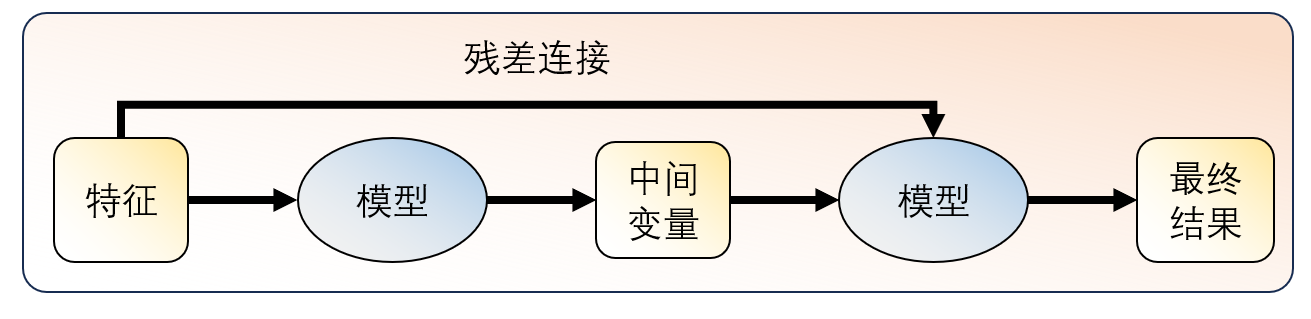
\includegraphics[width=0.7\linewidth]{figures/问题三流程}
	\caption{数据流向图}
	\label{fig:}
\end{figure}



基于以上分析,构建双层预测模型,上层预测输入特征值,输出目标变量num\_ppdu和ppdu\_dur;再将目标变量num\_ppdu和ppdu\_dur作为特征输入,构建吞吐量的下层预测模型。该层次预测模型所选用的上层特征如下表所示。

\begin{table}[H]
	\centering
	\caption{特征值(部分)}
	\begin{tabular}{ccccc} % 
		\toprule
		SINR & protocol & signal\_quality &  per & eirp\\ 
		\midrule
		30.064 & 20 & -72.2375 &  0.27 & 13 \\
		25 & 20 & -83.975 &  0.15 & 9 \\
		25 & 8 & -83.975 &  0.14 & 9 \\
		25.6628 & 20 & -83.8 &  0.17 & 10 \\
		43.6236 & 20 & -82.5389 &  0.03 & 10 \\
		\bottomrule
	\end{tabular}
\end{table}

上层预测模型输出num\_ppdu和ppdu\_dur后,同步更新下层输入特征,共计7类。经过5重交叉验证和网格搜索调参后,该层次预测模型的整体最优参数组合如下表所示。


\begin{table}[H]
	\centering
	\caption{最佳得分和参数设置}
	\begin{tabular}{cc}
		\toprule
		指标 & 最佳值/参数设置 \\
		\midrule
		最佳得分 (Best Score) & 0.8421 \\
		学习率 (Learning Rate) - 梯度提升 & 0.05 \\
		基学习器数量 (N\_estimators) - 梯度提升 & 100 \\
		最大深度 (Max Depth) - 随机森林 & 10 \\
		基学习器数量 (N\_estimators) - 随机森林 & 200 \\
		惩罚参数 (C) - 支持向量回归 & 10 \\
		核函数 (Kernel) - 支持向量回归 & `rbf' \\
		\bottomrule
	\end{tabular}
\end{table}


\begin{table}[H]
	\centering
	\caption{优化后的层次Stacking模型性能}
	\begin{tabular}{@{}cccc@{}}
		\toprule
		 均方误差 (MSE) & 均方根误差 (RMSE) & 平均绝对误差 (MAE) & 决定系数 (R²) \\
		\midrule
		 303.6069 & 17.4243 & 11.9287 & 0.9078 \\
		\bottomrule
	\end{tabular}
\end{table}

如表7.15所示,优化后的层次Stacking 模型在 MSE、RMSE 和 MAE 上表现良好,误差较小。同时,R² 值接近 1,显示出模型的高拟合度和解释能力。因此,该模型在处理吞吐量时具有很好的预测性能。

\begin{figure}[H]
	\centering
	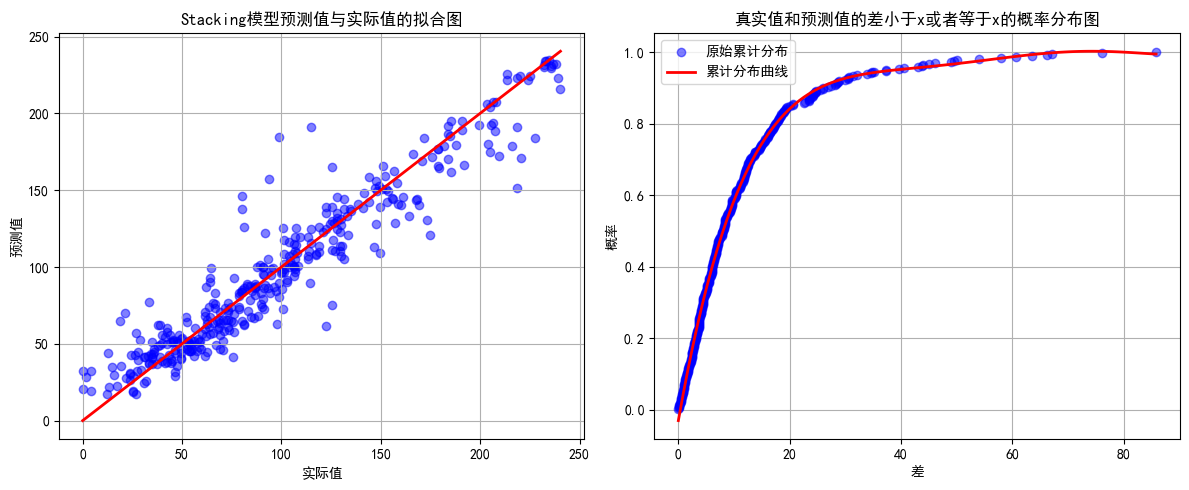
\includegraphics[width=0.8\linewidth]{figures/问题三888}
	\caption{模型预测性能图}
	\label{fig:888}
\end{figure}



如图7.19所示,层次Stacking 模型的残差分布近似正态分布,大量测试集的误差处于[ -10,+10 ]之间,平均绝对误差为11.9,稳定性较好,模型的预测精度较高。